\documentclass[12pt,a4paper]{article}
\usepackage[swedish,english]{babel}
\usepackage[T1]{fontenc}
\usepackage[utf8]{inputenc}
\usepackage{graphicx}
\usepackage{mathtools}
\usepackage{subcaption}
\usepackage{float}
\usepackage{footnote}
\usepackage[toc,page]{appendix}

\graphicspath{ {images/} }

\makesavenoteenv{tabular}

\author{
  Matstoms, Axel
  \and
  Jankovi\'{c}, Luka
  \and
  Matstoms, Ivar
}

%\date{2018-03-15}

\title{Tolkning och förenkling av matematiska uttryck i form av en symbolhanterare}

\begin{document}
\selectlanguage{swedish}
\maketitle
\begin{figure}[h]
  \centering
  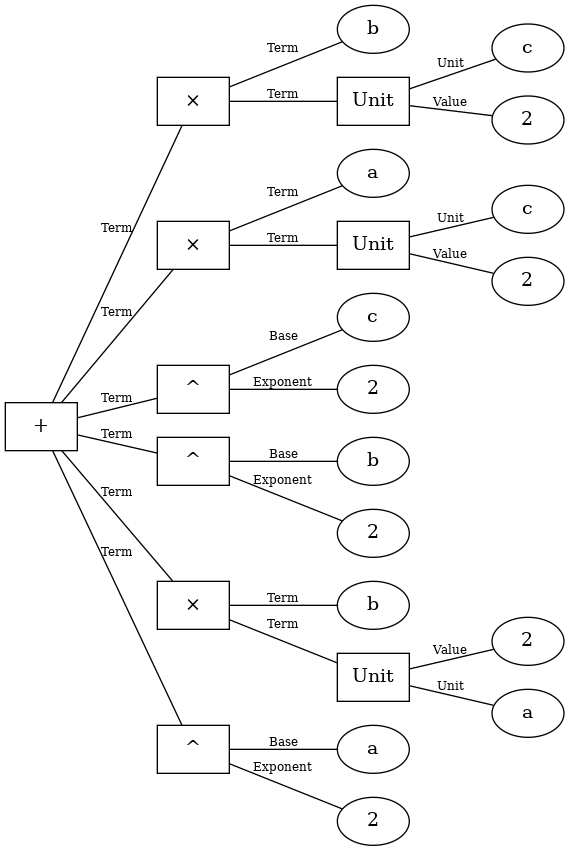
\includegraphics[width=0.6\textwidth]{image27}
  %\caption{Välj en olämplig bild}
\end{figure}
\begin{center}
  \textbf{Handledare: }Mikael Rydfalk\\
  \textbf{Medbedömare: }Thomas Lejdå
\end{center}
\newpage
\selectlanguage{english}
\begin{abstract}
The purpose of this project is to look at some of the techniques used by sites such as WolframAlpha to simplify algebraic expressions and solve particular kinds of equations. To research this we wrote an application in Python with some of the features of such sites.  We chose to work with Python due to its simplicity and due to the fact that everybody in the group knew it before the project even started. During the span of this project we were able to develop an application which is able to take input and construct an abstract syntax tree which is then simplified. The application is able to handle many of the goals that were set in the beginning of this project, including addition and multiplication of polynomials correctly, although not always fully simplified. The application is also able to solve polynomial equations up to and including the second degree. With time the application could easily be expanded to cover more aspects of what we set out to do such as polynomial division and solving polynomial equations of higher grades.
\end{abstract}
\textbf{Keywords:} Abstract syntax tree; Python; Algebraic Expressions
\selectlanguage{swedish}
\newpage
\tableofcontents
\newpage
\section{Inledning}
Eftersom vi alla i gruppen delar en stor passion för programmering ville vi göra ett arbete som involverar både programmering och ett naturvetenskapligt ämne. Vi övervägde flera olika idéer, bland annat en realtids fysikmotor, implementationer av matematiska funktioner (såsom sinus, exponenter) på hårdvarunära nivå samt idén som valdes: att skriva en symbolhanterare vid namn GAMLP (\textbf{G}a-\textbf{A}rbete \textbf{M}atematikbib\textbf{L}iotek i \textbf{P}ython). En symbolhanterare, eller CAS, Computer Algebra System, är ett datorprogram som kan tolka och lösa ekvationer, exempelvis \(5x + 10 = 20\). En annan funktion som en symbolhanterare har är förmågan att förenkla uttryck, exempelvis \((x + 2)(x - 3) \Leftrightarrow (x^{2} - x - 6)\). Skillnaden mellan en vanlig miniräknare och en symbolhanterare är att symbolhanterare förstår algebra samt att en symbolhanterare kan hantera variabler, inte bara värden. 
\par
Syftet med arbetet är att undersöka hur verktyg såsom WolframAlpha fungerar, dvs. hur inmatad data tolkas, hanteras och förenklas och utifrån det skriva ett bibliotek som kan förenkla uttryck och lösa ekvationer. Arbetet har utgått från följande frågeställningar:
\begin{itemize}
	\item Hur kan inmatad data representerad som trädstruktur tolkas och arbetas med av ett program?
	\item Hur kan uttryck förenklas m.h.a. dessa trädstrukturer?
	\item Hur kan algoritmer användas för att lösa ekvationer?
\end{itemize}
\section{Teori}
För att tolka ekvationer som är skrivna på vanlig form (e.x. \(5x + 10 = 15\)) måste de representeras med hjälp av en datastruktur. Detta underlättar processen att skriva algoritmer som kan förstå strukturen av en ekvation och utföra förenklingar.
\subsection{Träd som datastruktur}
\label{subsec:trees}
Inom datavetenskap beskrivs träd som en form av graf som används för att representera hierarkisk data. Ett träd inom matematiken består av noder som är sammansatta på så vis att varje nod kan innefatta ett eller flera barn, som i sig också är noder. I det här dokumentet kallas barnen för subnoder. En subnods ``förälder'' kallas just så: förälder. Noder behöver dock ej innefatta några subnoder, dessa noder kallas för löv. Varje nod behöver dock anta ett värde. Om en nod inte har en förälder betyder det att denna nod är högst upp i trädet. Denna nod kallas för rotnod eller bara rot.
\subsubsection{Abstrakt syntaxträd}
Abstrakta syntaxträd är träd som representerar syntaxen av t.ex. ett språk. Det som gör trädet abstrakt är att det inte tar hänsyn till t.ex. parenteser eller mellanrum (Ranta, 2011). Abstrakta syntaxträd används oftast inom datavetenskap för att strukturera programmeringskod så att en kompilator kan omvandla källkoden till ett exekverbart program. Men på grund av likheterna mellan programmeringsspråkens syntax och matematiska ekvationer användes abstrakta syntaxträd i detta arbete.
\subsection{Multinomialsatsen}
För att utveckla potenser av multinom (e.x. \((a + b + c)^{3}\)) används multinomialsatsen. Som man kan ana på namnet liknar multinomialsatsen binomialsatsen. Skillnaden är att multinomialsatsen är ett mer generaliserat sätt att beskriva utveckling av polynom, och är alltså ej begränsad till endast binom. Satsen lyder
\[(a_{1}+a_{2}+\ldots+a_{m})^{n}=\displaystyle\sum_{k_{1}+\dots+k_{m}=n}\binom{n}{k_{1},k_{2},\dots,k_{m}}a_{1}^{k_{1}}\cdot\ldots\cdot a_{m}^{k_{m}}\]
Den behöver dock lite förklaring. Med \(\displaystyle\sum_{k_{1}+\dots+k_{m}=n}\) menas alla möjliga kombinationer med återläggning av exponenter i \(a_{1}^{k_{1}}\cdot a_{2}^{k_{2}}\cdot\ldots\cdot a_{m}^{k_{m}}\) där \(\displaystyle\sum_{i=0}^{m}k_{i}=n\) uppfylls. Vidare behöver  \(\binom{n}{k_{1},k_{2},\ldots,k_{m}}\) förklaras. Detta kallas för \textit{multinomialtal} eller \textit{multinomialkoefficient}, som i sig en generalisering av binomialkoefficienten \(\binom{n}{k}\). Multinomialkoefficienten kan skrivas om på detta vis.
\[\binom{n}{k_{1},k_{2},\ldots,k_{m}}=\frac{n!}{k_{1}!\cdot k_{2}!\cdot\ldots\cdot k_{m}!}\]
%exempel

\subsection{Klasser och Objekt}
\label{subsection:klasserochobjekt}
En viktig del av struktureringen av noder handlar om att en nod kan vara en utvidgad (eng. extended) typ av en annan nod. Det vill säga, istället för att på nytt skapa varje nod kan man istället skapa en allmän nod för t.ex. operatörer, och sedan utvidga den för varje sorts operation. Detta kallas för Objektorienterad Programmering (\textbf{O}bject \textbf{O}riented \textbf{P}rogramming, OOP). 
\subsubsection{Objektorienterad programmering}
\label{subsubsection:oop}
Objektorienterad programmering funkar genom att man för varje föremål, struktur, etc. man vill beskriva i ett program har en s.k. klass. En klass är en abstrakt modellering av ett objekt; dvs. den innehåller definitioner för egenskaper och funktioner. (Kan t.ex. liknas vid en ritning; klassen innehåller information om strukturen, men är i sig inte en färdig produkt.). Sedan används klassen för att skapa objekt som kan fylla på med värden på attributerna och faktiskt utföra de beskrivna handlingarna. Ett exempel är att föreställa sig klassen Bil. I denna klass är det definierat att varje bil har t.ex en färg, maxhastighet, osv. Den har också vissa handlingar (alt. metoder) beskrivna; man kan köra bilen, tanka den, osv. Detta är beskrivningen av klassen Bil, och det är väldigt viktigt att komma ihåg att klassen, dvs. definitionen av bilen i sig ej är en bil. Istället skapas en instans av klassen bil; alltså kan man säga att objektet är skapat med klassen som ritning. Vi återvänder till Bil-exemplet och skapar ett objekt; en bil med färgen blå och maxhastighet 200 km/h. Denna teoretiska bil kan nu köras, tankas osv.
\subsubsection{Subklasser och arv}
Ett användbart redskap inom objektorienterad programmering är arv. För att fortsätta med bil-exemplet kan vi säga att klassen Bil är en subklass (dvs ärver från) klassen Fordon. Klassen Bil har då alla attributer och metoder som klassen Fordon har samt attributer och metoder som läggs till i definitionen av Bil. Klassen fordon kan exempelvis ha attributerna kan-flyga och bränsle-typ. Därmed kan en instans av klassen Bil anta värden för dessa attributer.
\section{Metod}                                                                
\subsection{Implementation av syntaxträd}
Trädet utgår från en rotnod. Om trädet representerar en ekvation är denna nod alltid ett likhetstecken. Likhetsnoden kan bara anta två subnoder, en för VL och en för HL. Därefter kan leden byggas upp av olika slags noder. Om trädet representerar ett uttryck kan rotnoden vara precis vilken slags nod som helst bortsett från likhetstecken, då skulle ju trädet representera en ekvation!
\subsection{Noder}
\label{subsubsec:noder}
Varje nod måste anta ett värde. Med detta menas ett numeriskt värde (e.x. \(5\) eller \(10\)), eller en operator (e.x. \(+\), \(-\), \(\cdot\), \(\div\), \string^). Alla nummernoder och okända blir löv i trädstrukturen. Alla andra sorters noder kräver subnoder, eftersom man givetvis inte kan bygga upp ett uttryck med enbart operatörer. Se Figur \ref{fig:2131} för ett exempel på hur ett uttryck kan representeras med hjälp av en trädstruktur.
\begin{figure}[H]
	%24
	\centering
	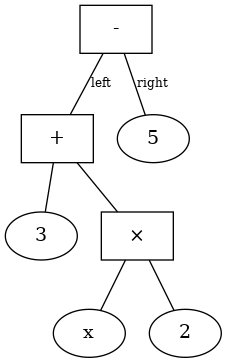
\includegraphics[width=0.3\textwidth]{image24}
	\caption{Visuell representation av \((2x + 3) - 5\) som ett abstrakt syntaxträd.}
	\label{fig:2131}
\end{figure}
\paragraph{Operatörsnoder}
Operatörsnoder är noder som representerar operationer och kräver därför subnoder. Exempel på operatörsnoder är additionsnod, som representerar addition mellan två eller flera noder och divisionsnod, som representerar division mellan två noder.
\paragraph{Homogena och inhomogena operatörsnoder}
\label{subsec:operator}
Homogena operatörsnoder representerar operationer där ordningen av värdena ej spelar någon roll, exempelvis \(a + b + c = b + c + a\). Detta betyder att homogena noder inte behöver ha en strikt vänsternod och högernod, utan kan istället lagra subnoderna som en lista. Därmed kan en operatörsnod ha ett godtyckligt antal subnoder. Inhomogena operatörsnoder representerar operationer där ordningen spelar roll, som t.ex. minus (\(a - b \neq b - a\)). Detta betyder att inhomogena operatörsnoder endast kan ha två subnoder, eftersom när dessa representeras som en trädstruktur kan går det inte urskilja mellan t.ex. \(a - b - c\) och \(a - c - b\).
\paragraph{Enhetsnoder}
Eftersom programmet ska kunna hantera ekvationslösning, måste okända variabler kunna representeras (e.x. \(5x + 10 = 20\). Här är \(x\), en okänd varaibel.) För att representera variabler används en speciell typ av nod: en så kallad enhetsnod. Denna nod antar ett värde för koefficienten och en representation av den okända variabeln, en så kallad enhet. Denna enhet består av själva variabeln och vilken grad som den representeras i. Se Figur \ref{fig:2132} för en visuell representation av \(2x^{2}\) som en enhetsnod.
\begin{figure}[H]
	%25
	\centering
	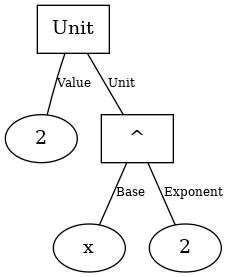
\includegraphics[width=0.3\textwidth]{image25}
	\caption{\(2x^{2}\) representerat som en enhetsnod med enheten \(x^{2}\) och värdet \(2\). Med \textit{Unit} menas enhet.}
	\label{fig:2132}
\end{figure}
\subsubsection{Noder representerade som klasser}
Alla noder är subklasser av klassen Nod. Nodklassen innehåller definitioner för funktioner som används av och är gemensamma för alla subklasser. T.ex. så hanteras operationer av noder (e.x. addition, subtraktion) av denna klass. (Inte själva förenklingen men helt enkelt skapandet av en operatörsnod med subnoder.) Alla operatörsnoder är subklasser av klassen operatörsnod. Operatörsnoden har dock ingen funktion i sig, utan används för att enklare urskilja vilka noder som är operatörsnoder och vilka som inte är. Därefter grupperas additionsnodens och multiplikationsnodens klass som var sin subklass av klassen honomgen operatörsnod. Detta gjordes eftersom både multiplikationsnoden och additionsnoden är homogena noder.
\begin{figure}[H]
  \center
  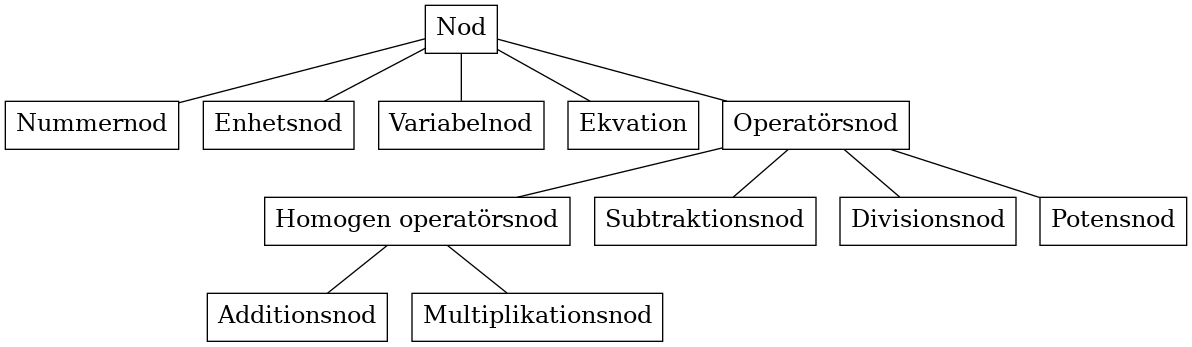
\includegraphics[width=1\textwidth]{image20}
  \caption{Diagram av nodklassen samt dess alla subklasser.}
\end{figure}

\begin{figure}[h!]
  \centering
  \begin{tabular}{l|p{10cm}}
    \textbf{Namn} & \textbf{Användning} \\
    \hline
    \texttt{hash\_node} & Returnerar ett unikt nummer för just denna nod som används för att identifiera den. \\
    \texttt{get\_children} & Returnerar subnoder. \\
    \texttt{get\_int\_value} & Om noden går att räkna ut och resultatet är ett heltal returnera heltalet. \\
    \texttt{latex} & Returnerar en latex representation. \\
    \texttt{simplified} & Bygger upp en nod som är en förenkling av sig själv. \\
    \texttt{eval} & Räknar ut värdet på en nod. \\
    \texttt{eq} & Jämför noder (samma struktur, variabler etc.) \\
    \texttt{formatted} & Returnerar en text representation av noden.
  \end{tabular}
  \captionof{table}{Funktioner och dess användning i basklassen nod.} \label{tab:basenodefunc}
\end{figure}

\subsection{Tolkning av inmatade ekvationer}
För att läsa in uttryck på normal form och för att enkelt omvandla de till abstrakta syntaxträd krävs en lexikalisk analys av den inmatade datan som sedan tolkas av en parser. Att hantera lexikalisk analys och att utveckla en parser ligger utanför projektet. Därför användes biblioteket purplex, som utför denna lexikaliska analys och har en inbyggd parser.

\subsubsection{Lexikalisk analys}
\label{subsubsec:lexikaliskanal}
En lexer separerar den inmatade datan till s.k. tokens baserat på fördefinierade mönster och bygger upp en array (lista) baserad på dessa tokens. Med andra ord letar en lexer efter ett sorts mönster i indatan och fyller på array-en med motsvarande tokens. Tokens känns igen med hjälp av mönstermatchningsspråket regex. Nedan visas en tabell över vilka mönster som letas efter och vad de ersätts med i listan i den lexikaliska analysen. 
Exempel: \(5x+10=20\Rightarrow\) ([värde, 5], [okänd, \(x\)], [addition], [värde, 10], [likhetstecken], [värde, 20])

\begin{figure}[h!]
  \centering
  \begin{tabular}{l|l}
    \textbf{Mönster} & \textbf{Tokens} \\
    \hline
    Nummer & Nummernod \\
    Bokstav & enhetsnod med värdet 1 \\
    Nummer och bokstav & Enhetsnod med värdet nummer \\
    \texttt{+} & Additionsnod \\
    \texttt{-} & Subtraktionsnod \\
    \texttt{*} & Multiplikationsnod \\
    \texttt{/} & Divisionsnod \\
    \texttt{\string^} & Potensnod \\
    \texttt{=} & Ekvation
  \end{tabular}
  \captionof{table}{Vilka mönster som letas efter i indatan och vad de ersätts med i den lexikaliska analysen.}
  \label{tab:lexer_patterns}
\end{figure}

\subsubsection{Parser}
Parserns (svenska - tolk) uppgift i vårt projekt är att bygga upp ett syntaxträd av listan som skickades över från den lexikaliska analysen\footnote{Se \ref{subsubsec:lexikaliskanal} Lexikalisk analys}. Eftersom det är då strukturen på ekvationen byggs upp är det viktigt att räknesätten prioriteras på rätt sätt. Ordningen på räknesätten är förutbestämt i regler som parsern följer. När tokens definieras anges också vilken ordning de ska prioriteras.

\subsection{Förenkling}
Operatörsnoder vars subnoder endast består av numeriska värden räknas helt enkelt ihop med den operatorn som noden representerar. Då kommer denna operatörsnod ersättas med en nummernod som antar det ihopräknade värdet.
\subsubsection{Homogena operatörsnoder}
\label{subsec:homogena}
När man matar in ett uttryck i programmet skapas först ett träd där alla operatörsnoder har två subnoder, se Figur \ref{fig:2311}.
\begin{figure}[H]
  %22
  \centering
  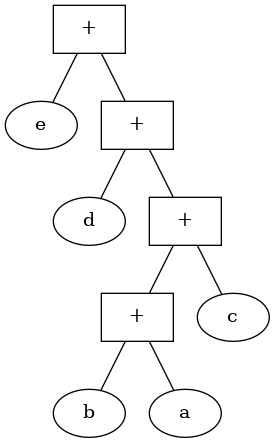
\includegraphics[width=0.3\textwidth]{image22}
  \caption{\((a + b + c + d + e)\) tolkat av programmet.}
  \label{fig:2311}
\end{figure}
Första steget i förenklingen är att ``platta ut'' ett träd av homogena noder av samma typ till en enda nod, se Figur \ref{fig:2312}. Subnoder med ett numerisk värde separeras från övriga subnoder och räknas ihop. Övriga subnoder som sammanfogas i största möjliga utsträckning. Ett exempel på en sammanfogning är \(x + x = 2x \). Exakt hur subnoder sammanfogas beror på nodens typ.
\begin{figure}[h!]
  %16
  \centering
  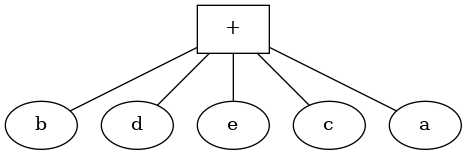
\includegraphics[width=0.5\textwidth]{image16}
  \caption{\((a + b + c + d + e)\) efter första steget av förenkling av homogen nod}
  \label{fig:2312}
\end{figure}
\paragraph{Additionsnod}
Nummeriska värden summeras, \(5 + 10 \Rightarrow 15\) och enhetsnoder kombineras genom att dess koeficient sätts baserat på antalet, exempelvis \(x + x + x = 3x\), eller \(5x + 3x = 8x\), se Figur \ref{fig:2321}.
\begin{figure}[H]
  \centering
  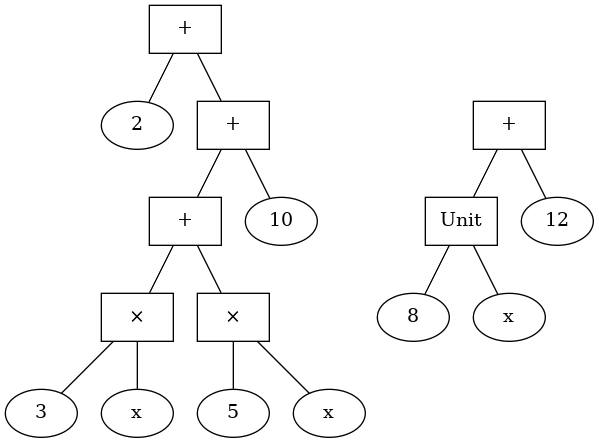
\includegraphics[width=0.7\textwidth]{image-merged2}
  \caption{\(5x + 3x + 10 + 2\) förenklas till \(8x + 12\)}
  \label{fig:2321}
\end{figure}
\paragraph{Multiplikationsnod}
%x^a * x^b = x^(a+b)
Om additionsnoder multipliceras kommer dessa lösas ut genom att kombinationer av additionsnodernas subnoder adderas. Därefter multipliceras resten av multiplikationsnodernas subnoder med summan av kombinationerna.
\[ \left( a+b \right) \cdot \left( c+d \right) \cdot ef \]
\[ \Leftrightarrow \]
\[ (ac + ad + bc + bd)\cdot ef \]
\[ \Leftrightarrow \]
\[ acef + adef + bcef + bdef \]
Enhetsnoder med samma okänd kombineras genom att skapa en ny enhetsnod där enheten blir produkten av de enheterna för noderna och koefficienten produken av koefficienterna (e.x. \(5x \cdot 10x = 50x^{2}\)). Enhetsnoder kan också kombineras med övriga noder genom att multiplicera in i enhetsnodens koefficient.\par
En potensnod kan slås ihop med en annan nod om basen på potensnoden är samma som den andra noden, isåfall skapas en ny potensnoden med exponenten ökad med ett.
\begin{figure}[H]
  \centering
  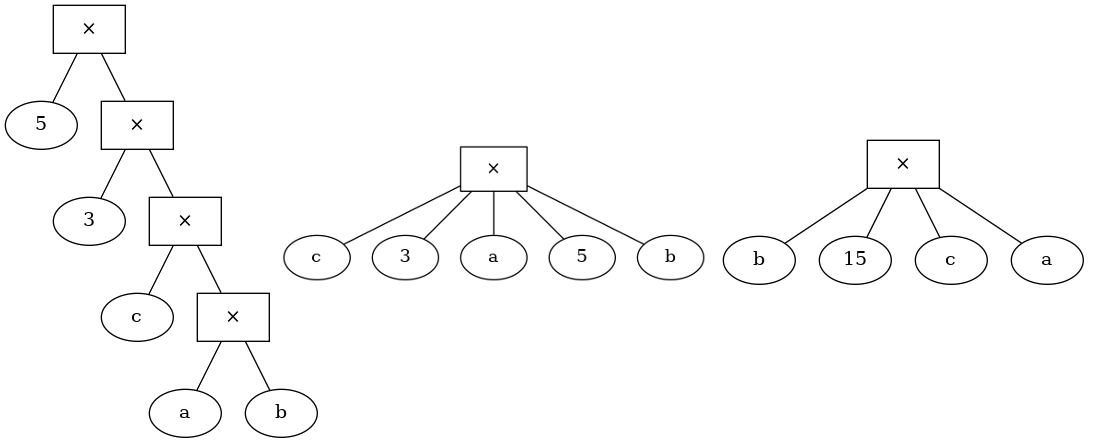
\includegraphics[width=0.9\textwidth]{image-merged}
  \caption{\((a \cdot b \cdot c \cdot 3 \cdot 5)\) förenklas i tre steg, a,b,c lyfts upp till samma nod och talen separeras till sin egen nod, tillslut räknas talen ihop.}
  \label{fig:2313}
\end{figure}
%behöver fixas
\begin{figure}[H]
  %26
  %32
  \centering
  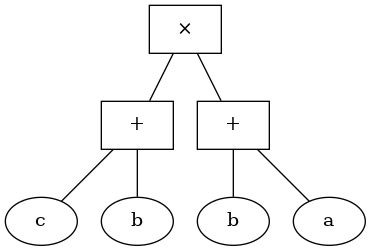
\includegraphics[width=0.4\textwidth]{image26}
  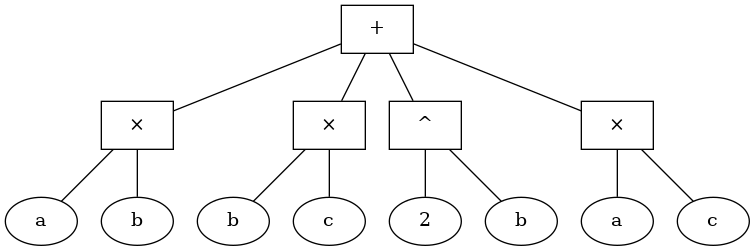
\includegraphics[width=0.8\textwidth]{image32}
  \caption{\((a + b) \cdot (c + b)\) förenklas till \((a \cdot b) + (b \cdot c) + (b ^ 2) + (a \cdot c)\)}
\end{figure}
\subsubsection{Inhomogena noder}
\paragraph{Potensnod}
\label{subsubsec:potensnod}
Potensnoder innehåller två subnoder, basen och exponenten. En potensnod kan ha vilken sorts nod som helst som basnod (bortsett från ekvationsnod), exempelvis \((a+b+c)^{3}\), där basnoden är en additionsnod. Om basnoden är en additionsnod kommer hela potensnoden förenklas m.h.a. multinomialsatsen, annars kommer basnoden förenklas separat, innan potensnoden förenklas. En potensnod med potens noll förenklas till en nummernod med värdet ett. 
\paragraph{Subtraktionsnod}
Subtraktionsnoden är ej en homogen nod då ordningen på termerna spelar roll, \(a-b\neq b-a, a \neq b\). Därmed måste subtraktionsnoden anta endast två subnoder; en för vänster term och en för höger term. För att förenkla subtraktionsnoden används additionsnoden och multiplikationsnoden för att uppnå en minusoperation. Istället för att direkt räkna ut \(a-b\) så skrivs uttrycket om till \(a+((-1)\cdot b)\). Därmed kan samma resultat uppnås med bara addition och multiplikation.
\begin{figure}[h!]
  \centering
  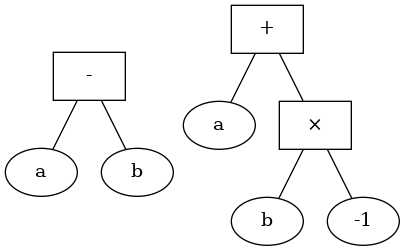
\includegraphics[width=0.5\textwidth]{image-merged3.png}
  \caption{\(a-b\) före och efter förenkling. Minus noden transformeras till en additionsnod med b ersatt med \(b \cdot -1\)}
\end{figure}
\paragraph{Divisionsnod}
\label{subsubsec:divnode}
På samma sätt som subtraktionsnoden skiver om uttrycket till en additionsnod så skriver divisionsnoden om uttrycket så att förenklingen istället kan hanteras av multiplikationsnoden och potensnoden. \(\frac{a}{b}\Rightarrow a \cdot \left(b^{-1}\right)\)
\begin{figure}[h!]
  \centering
  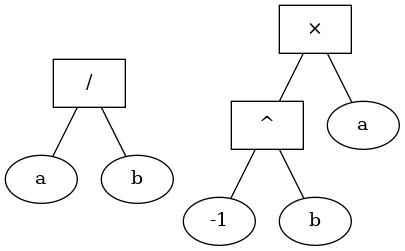
\includegraphics[width=0.5\textwidth]{image-merged4.png}
  \caption{\(\frac{a}{b}\) förenklas till \(a \cdot \left(b^{-1}\right)\)}
\end{figure}
\paragraph{Kvadratrotnoder}
\label{subsubsec:sqrtnod}
För att förenkla kvadratrotsnoder skrivs de om till potensnoder. \(\sqrt{x}=x^{\frac{1}{2}}\)
\begin{figure}[h!]
  \centering
  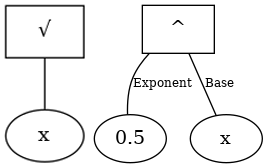
\includegraphics[width=0.4\textwidth]{sqrt.png}
  \caption{\(\sqrt{x}\) förenklas till \(x^{\frac{1}{2}}\)}
\end{figure}
\subsection{Ekvationslösning}
En ekvation löses genom att först subtrahera högerledet från båda led så att högerledet blir 0. Mer specifikt skapas en subtraktionsnod med båda leden som subnoder, som därefter förenklas. 
\par Detta leder till att ekvationen kan lösas med en allmän metod som väljs beroende på vilken grad ekvationen är av. Vilken grad ekvationen är av bestäms enhetsnoden med högst potens.
\subsubsection{Ekvationsmetoder}
Dessa metoder används för att bestämma värdet på en enhetsnod från en ekvation.
\label{subsubsec:Ekvationsmetoder}
\paragraph{Förstagradsekvationer}
\(kx+m=0\Leftrightarrow x=\frac{-m}{k}\)
\paragraph{Andragradsekvationer}
\(ax^{2}+bx+c=0\Leftrightarrow x=-\frac{b}{2a}\pm \sqrt{\frac{b^{2}}{(2a)^{2}}-\frac{c}{a}}\)
\paragraph{Enkla exponensialekvationer}
\(a\cdot x^{b}+k=0\Leftrightarrow x=(\frac{-k}{a})^{\frac{1}{b}}\)

\subsection{Bilder på träd}
Bilderna på träden som används relativt ofta i denna rapport är också del av GAMLP, som har möjligheten att generera bilder av träd. Dessa genereras med hjälp av biblioteket \textit{graphviz}. För varje träd går programmet igenom trädet uppifrån och ner och skapar listor med alla noder och kanter. Programmet beskriver sedan kod med dotsyntax, som sedan tolkas med programmet dot för att generera en bild på trädet.

\subsection{Källor}
\subsubsection{Struktur}
Strukturen av projektet baserades till viss del på ett examensarbete vid namn \textit{Constructing a Computer Algebra System Capable of Generating Pedagogical Step-by-Step Solutions} skriven av Dimitrij Lioubartsev (KTH, 2016). Syftet med detta examensarbete är att modifiera ett existerande bibliotek för symbolhantering, SymPy, så att det kan generera stegen som krävs för att kunna lösa en ekvation. Detta var givetvis ej syftet med vårt gymnasiearbete, men examensarbetet gick in i detalj hur en symbolhanterare kan fungera (kapitel 3). Denna text användes som källa då den kändes relevant till vårt arbete. Vi kunde använda källan för inspiration för hur arbetet skulle läggas samt som exempel på hur själva rapporten kunde se ut.

\subsubsection{Multinomial}
Förenkling av uttryck på formen \((x_{1}+x_{2}+...+x_{k})^{m}\) görs med multinomialsatsen. Då vi endast jobbat med ett specialfall av den här formen på uttryck, binomial, behövde vi hitta ett sätt att förenkla uttryck på den allmänna formen. Sidan om Multinomial Theorem på Proof Wiki var till stor hjälp och kunde även verifieras mot Encyclopædia Britannicas sida om samma ämne. Proof Wikis sida innehöll mer information och var till större nytta.

\section{Resultat}
Programmet innefattar nu dessa förmågor:
\begin{itemize}
	\item Representera inmatad data som syntaxträd
	\item Rekursivt förenkla operationer samt korrekt kunna hantera okända variabler för att förenkla uttryck.
	\item Lösa ut okända variabler från ekvationer genom att använda olika metoder för olika ekvationsgrad.
\end{itemize}

\subsection{Vad kan biblioteket hantera}
\subsubsection{Förenkling av uttryck}
Programmet strävar efter att förenkla ekvationen så den blir omskriven på polynomform, vilket kan vara fördelaktigt i vissa situationer, dock inte alla. Exempelvis för ekvationen \((x-3) \cdot (x-5)=0\) är det uppenbart att rötterna är \(x=3, x=5\) men i polynomform \(x^{2}-8x+15=0\) blir ekvationen lite svårare att lösa. I det här fallet skulle programmet fortfarande kunna lösa ekvationen i polynomform, men om ekvationen var av tredje graden eller högre skulle detta inte vara fallet.
\begin{savenotes}
\begin{figure}[H]
  \centering
  \begin{tabular}{l|l}
    \textbf{Uttryck} & \textbf{Förenklas till} \\
    \hline
    \(\frac{ac + bc}{c}\) & \(a+b\) \\
    \(a+a\) & \(2a\) \\
    \(a \cdot a\) & \(a^{2}\) \\
    \(a - a\) & \(0\) \\
    \((a+b)^{2}\) & \(a^{2} + 2ab + b^{2}\) \\
    \(\frac{a}{a}\) & 1 \\
    \((a+b+\ldots)^{k}\) & Utvecklas m.h.a. multinomialsatsen \\
    \(ak+am\) & \(a(k+m)\) \\
    \(\frac{a+b}{c+d}\) & Programmer kraschar
  \end{tabular}
  \captionof{table}{Uttryck och vad de förenklas till (om möjligt)}
  \label{tab:expressions}Vissa saknas
\end{figure}
\end{savenotes}

\subsubsection{Ekvationslösning}
Programmet kan lösa relativt avancerade ekvationer. Programmet är i första hand utvecklat för att lösa polynomekvationer.

\begin{figure}[h!]
  \centering
  \begin{tabular}{l|l}
    \textbf{Allmänt uttryck} & \textbf{Löser programmet ekvationen?} \\
    \hline
    \(ax+b=0\) & Ja \\
    \(\frac{x}{a}=b\) & Ja \\
    \(ax^2+bx+c=0\) & Ja \\
    \(\frac{a \cdot x^2}{b}+\frac{x \cdot c}{d}+\frac{e}{f}=g\) & Ja \\
    \((x+a)(x+b)=c\) & Ja \\
    \(\frac{(x+a)\cdot(x+b)}{c}+d=e\) & Ja \\
    \(x^a+b=c\) & Endast om \( a>0 \) \\
    \((x+a)\cdot(x+b)\cdot(x+c)=d\) & Nej 
  \end{tabular}
  \captionof{table}{Ekvationer och om de kan lösas}
  \label{tab:lexer_patterns}
\end{figure}

\subsection{Arbetsprocess}
\subsubsection{Python}
Vi valde att skriva programmet i programmeringsspråket Python då det är allmänt enkelt att förstå och att arbeta med. Dessutom hade vi alla kunskap inom språket innan vi började med projektet.

\subsubsection{Github}
Programmet sparades på GitHub, som är en service för versionshanteringsprogrammet git. Git underlättar programmeringsprocessen för projekt som innefattar flera deltagare. GitHub har också inbyggda funktioner för t.ex. problemhantering, då s.k. issues kan öppnas för att flagga upp utvecklarna att man har funnit ett eller flera problem i koden.

\section{Diskussion}
\subsection{Komplexitet}
\label{subsec:Komplexitet}
En kods komplexitet definieras som gränsvärdet av tiden det tar för programmet att utföra sin uppgift när storleken på indatan går mot oändligheten. Att komplexiteten är ett gränsvärde har fördelen att den endast blir beroende av det största värdet, dvs. indatan. Till exempel: om det tar linjär tid att ta indata och kvadratisk tid att behandla indatan blir komplexiteten kvadratisk tid då den linjära termen inte spelar någon roll när storleken på indatan blir hög/stor. Detta skrivs som \(O(n^2)\). Med \(O\) menas juste gränsvärdet när n går mot oändligheten.
\par
Även om projektet blev ett bibliotek som kan användas inuti andra program så fokuserade vi inte på att göra programmet så snabbt som möjligt. Det var viktigare för oss att få så många kärnfunktioner som möjligt att fungera bra så att biblioteket, m.h.a. ett program som är inkluderat i projektet, kan användas som en avancerad miniräknare. Eftersom sannolikheten att programmet kommer behöva hantera stora mängder indata är låg, är hastigheten på programmet inte direkt relevant vid dessa situationer. 
\subsection{Kodstruktur}
Kodstruktur är essentiellt för större projekt för att underlätta vidareutveckling. Därför delade vi upp projektet exempelvis i klasser. Under arbetets gång hjälpte det oss att förstå varandras kod.
\par
Strukturen var dock inte perfekt. Klasserna delades upp i varsin fil, och eftersom klasserna ofta behöver ha tillgång till andra klasser och dess metoder behöver dessa då importeras. Detta ledde till att om två klasser behövde tillgång till varandra (vilket hände i vårt fall) så skulle de importera varandra. Inom programmering kallas detta för circular import, och är allmänt dålig praxis, eftersom det ökar risken till att programmet helt enkelt inte funkar, eller att det t.ex. blir svårare att reorganisera projektet om det skulle behövas.
\subsection{Möjliga förbättringar}
Just nu kan biblioteket endast lösa ekvationer som är skrivna på polynomform, och endast upp till den andra graden. Dessvärre hanteras division på ett sätt som gör att vissa ekvationer (framförallt de som inkluderar division med en okänd variabel) ej går att lösas. Tyvärr inkluderar detta också trivialfallet \( \frac{x}{x} = 1 \). På grund av detta kan bibliotek ej heller utföra polynomdivision.
\par
Även om fokuset på projektet ej låg på hastigheten (se \ref{subsec:Komplexitet}) betyder det inte att det inte finns fördelar med att göra projektet snabbare, mer effektivt. Användningsområdet av biblioteket skulle utökas drastiskt, då det skulle kunna användas i applikationer som kräver förenkling av t.ex. polynom av någon hundratals grad.
\par
Biblioteket har också problem med att utföra konjugatregeln. För det mesta gör biblioteket rätt men det har problem med att förenkla \( ab + (-1) \cdot ab\).
\subsection{Lärdomar}
Vi har lärt oss essenserna av syntaxträd och hur man kan strukturera de, inklusive hur man kan specialisera olika noder så att de har olika funktioner. (Se \ref{subsubsec:noder}) Vi lärde oss också hur man med hjälp av programmeringsspråkets implementation av klasser och arv kan implementera det i ett bibliotek.
\par
Algoritmen för potensnoden krävde att vi skulle känna till multinomialsatsen; något som ingen av oss kände till innan projektet.

\section{Källkritik}
Det ligger i naturen hos mycket av den informationen vi använt oss av att den är väldigt lätt att verifiera. Antingen funkar en algoritm eller inte, det går inte att vinkla en algoritm. 
\subsubsection{KTH}
Examensarbetet är skrivet år 2016 av Dimitrij Lioubartsev, student vid KTH. Examensarbetet kontrollerades av handledare och därför kan vi vara säkra på att källan är pålitlig. Dessutom är KTH ett väldigt välrespekterat universitet.
\subsubsection{Chalmers}
Informationen hämtades från anteckningar av en föreläsning på Chalmers, 2011 för information om abstrakta syntaxträd. Föreläsningen hölls av professorn Aarne Ranta, som också är avdelningschef för funktionel programmering på Chalmers.
\subsubsection{Encyclopædia Britannica}
Encyclopædia Britannica är ett av om inte det mest respekterade uppslagsverken som finns. Informationen är skriven av experter och verifierad, det gör det till en bra källa. 
\subsubsection{Proofwiki}
Proofwiki är en wiki för matematiska bevis. För att skriva och ändra krävs godkännande, medlemskap söks inte skapas. Den är fortfarande overifierad med eftersom informationen överensstämmer med britannica.
\subsubsection{Python.org}
Python.org är skrivit av Pythons utvecklare, och det gör informationen extremt trovärdig. Dessutom är även den här typen av information antingen fungerande eller inte. 

\begin{thebibliography}{9}

\bibitem{kth}
  http://www.diva-portal.se/smash/get/diva2:945222/FULLTEXT01.pdf
  Dmitrij Lioubartsev,
  \textit{Constructing a Computer Algebra System Capable of Generating Pedagogical Step-by-Step Solutions},
  KTH,
  2016,
  [2017-10-21]

\bibitem{Britannica}
  https://www.britannica.com/science/multinomial-theorem
  William L. Hosch,
  \textit{Multinomial theorem},
  Britannica,
  [2018-02-18]

\bibitem{dotdoc}
  http://www.graphviz.org/pdf/dotguide.pdf
  \textit{Graphviz dot dokumentation},
  [2018-02-10]

\bibitem{chalmers}
  http://www.cse.chalmers.se/edu/year/2011/course/TIN321/lectures/proglang-02.html
  Aarne Ranta,
  Chalmers,
  2011
  [2018-05-06]

\bibitem{pythondoc}
  https://docs.python.org/3/
  \textit{Python dokumentation},
  Python Software Foundation ,
  [2017-2018] 
\end{thebibliography}
\newpage
\begin{appendices}
\section{\\Begrepp}
\begin{figure}[h!]
  \centering
  \begin{tabular}{l|l|l}
    \textbf{Uttryck} & \textbf{Förklaring} & \textbf{Se} \\
    \hline
    Nod & En det av trädet & \ref{subsec:trees} \\
    Subnod & En nod under en annan nod & \ref{subsec:trees} \\
    Rotnod & Noden högs upp i trädet & \ref{subsec:trees} \\
    Homogena noder & Operatörsnoder där ordningen inte spelar någon roll(+,\(\cdot\)) & \ref{subsec:homogena} \\
    Inhomogena noder & Operatörsnoder där ordningen spelar roll(-,/) & \ref{subsec:homogena} \\
    Lexikalisk analys & Sepererar en text rad tex 'a+b' blir a,+,b & \ref{subsubsec:lexikaliskanal} \\
    Token & sv tecken, i detta fallet delar av ett utryck tex ett tal & \ref{subsubsec:lexikaliskanal} \\
    Parser & Gör om en lista av tokens till ett träd med avsende till prioritet & \ref{subsubsec:lexikaliskanal} \\
    Object & Har metoder och egenskaper & \ref{subsubsection:oop} \\
    Klass & Ritning för ett objekt & \ref{subsubsection:oop} \\
  \end{tabular}
\end{figure}
\section{\\Hur man använder biblioteket/programmet}
\subsection{\\Installationskrav}
\begin{itemize}
  \item GNU+Linux / BSD / macOS / termux(Android) / cygwin(Windows)
  \item Python 3
  \item Purplex
  \item PIL
\end{itemize}
\subsection{\\Valfria krav}
\begin{itemize}
  \item Graphviz
  \item Feh
\end{itemize}
\subsection{\\Installationsinstruktioner}
\begin{enumerate}
  \item Ladda ner GAMLPs källkod från github \begin{verbatim}$ git clone https://github.com/ALI-Team/GAMLP.git\end{verbatim}
  \item Kör installations skriptet setup.py (administratörs rättigheter kan behövas) \begin{verbatim}# python(3) setup.py install\end{verbatim}
\end{enumerate}
\subsection{\\Använding av programmet}
Biblioteket kommer med ett program för att enkelt kunna testa/använda det. Kör ``gamlp'' i terminalen för att starta det.\\
Utryck kan sedan direkt matas in i programmet som kommer bearbeta den inmatade datan utifrån olika regler, som i GAMLP kallas för \textit{flaggor}. Vilka flaggor som är tillgängliga fås av kommandot ``flags'' (exempel på flaggor kan vara t.ex. generera en bild på trädet.)  För att ändra på en flagga används kommandot ``set [namn] [on/off]''.
\end{appendices}
\end{document}
